\documentclass[12pt]{report}
\usepackage{snepospec}
\usepackage{ulem}
% TODO add snepo document imports
\begin{document}

\setlength{\headsep}{16pt}
\chead{Flash Tutorial}

\tableofcontents

\chapter{Getting Started}
\section{A Flash comments page}

\paragraph{}
``The Initech Flash site needs COMMENTS!'' your boss shouts. The
command bellows through the office and lands firmly on your
desk. ``Data Driven! RIA SPEEDWAGON! Oh, and can you do it by lunch?''
he follows with, frothing ever so slightly. Luckily you can. In about
fifteen minutes you can add a comments section to your Flash site,
leaving your lunch hour intact.
\paragraph{}
So give Lumberg a nod, tell him it will take at least three hours and
you may have to work through lunch but by gosh, you'll get it
done. You don't even have to send a Thank You note, just think of us
when you're spending the rest of the morning surfing ebay for antique
curling irons.

\section{Making sure you're set up and ready to go}

\subsection{Windows}
\begin{itemize}
\item Double click the \texttt{depot-VERSION.exe} file. This will start the
  Depot installer. Follow the on screen instructions.
\item Click \texttt{Start$\rightarrow$All Programs$\rightarrow$Snepo$\rightarrow$Depot$\rightarrow$start-web}
\item Click \texttt{Start$\rightarrow$All Programs$\rightarrow$Snepo
$\rightarrow$Depot$\rightarrow$start-depot-service}
\end{itemize}

\subsection {Mac}
\begin{itemize}
\item Open the \texttt{depot-VERSION.pkg} file. This will start the
  Depot installer. Follow the instructions, Depot will be installed
  under \texttt{/Users/YourName/depot}.
\item Open a terminal window
\item \texttt{cd path/to/depot}
\item \texttt{./start-web.sh \&}
\item \texttt{./start-depot.sh}
\end{itemize}

\subsection{Linux}
\begin{itemize}
\item \texttt{tar -xzvf depot.tar.gz}
\item \texttt{cd depot}
\item \texttt{./start-web.sh \&}
\item \texttt{./start-depot.sh}
\end{itemize}

When depot starts it examines the \texttt{depot.config}
file. The admin password is set using the value of the
\texttt{admin-password} parameter. Any user who is authenticated 
as an admin has unrestricted access to your Depot data store.
The default password is \texttt{cthulu}. If you change the password
in the config file restart Depot to load the new password.
We recommend changing the password before deploying to any public server.


\paragraph{}
If you want to make sure that you've properly set things up, after
depot is started point your browser at
\url{http://localhost:2323/depot/junk}. If things are working
correctly you will see a bunch of output like this:

\begin{center}
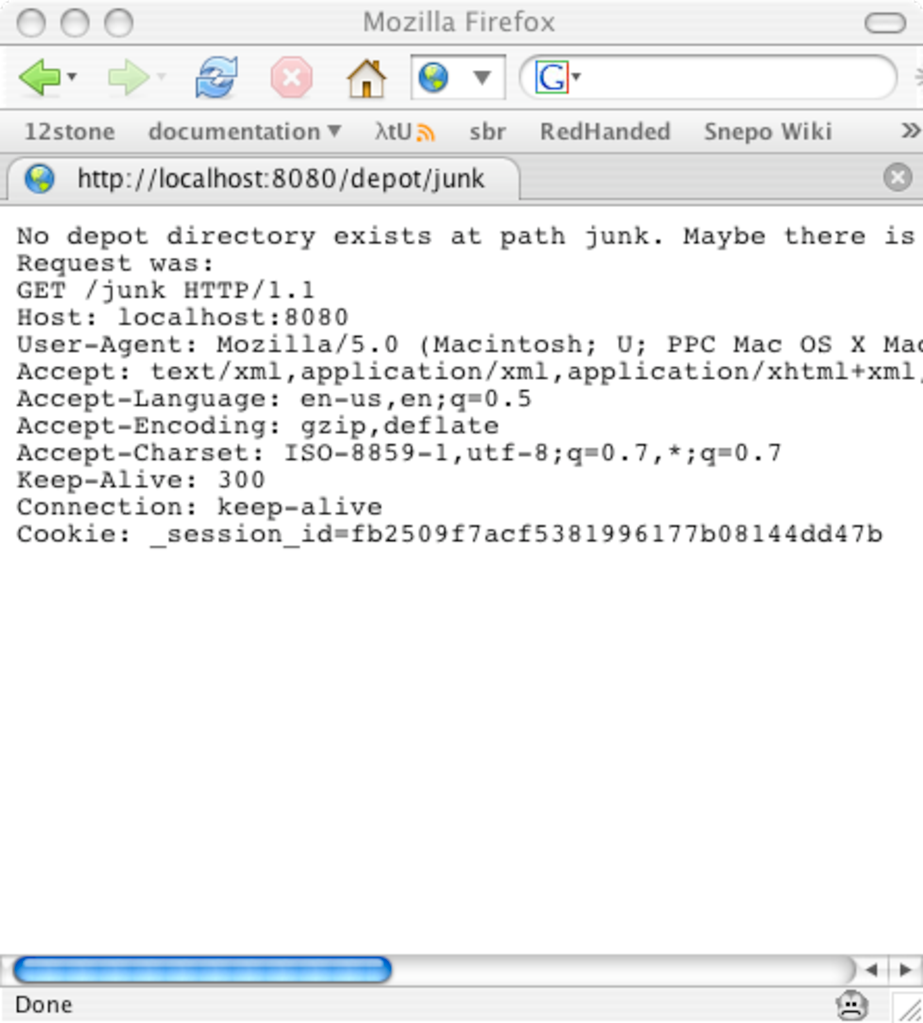
\includegraphics[scale=0.7]{wiki-tutorial-images/wiki-screenshot-404.pdf}
\end{center} 

\paragraph{}
Note that if you are using FireFox the output may not display in the
browser but you will be prompted to download a text file. 
\pagebreak

\chapter{Let the coding begin}
\section{Putting things on the timeline}
%\pullquote{ 

%  \textbf{CAUTION: COPY-PASTING FROM THE PDF DOESN'T ALWAYS WORK}. The
%  typesetting system that we use is brilliant for creating nice print
%  documents, however some characters will not paste properly and may
%  leave you scratching your head as to why the code doesn't
%  work. Watch out for quotes (single and double) and special
%  characters. If you want to save typing the source files are
%  available in your install directory under \texttt{web/flash}

%}
\paragraph{}
Now that depot is running let's build that flash page. Start by
putting together some assets on the timeline. First create a large
Multiline dynamic textfield on the main timeline. Give it the instance
name \texttt{commentsDisplay} and enable HTML. \texttt{commentsDisplay} 
is where the comments loaded from Depot will be populated.

\begin{center}
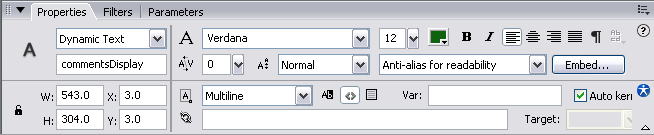
\includegraphics[scale=0.70]{flash-tutorial-images/usage-commentsDisplay-properties.png}
\end{center}

\paragraph{}
Next, create two text input fields. Make the first one a
Single Line input textfield and give it the instance name
\texttt{nameInput}.


\begin{center}
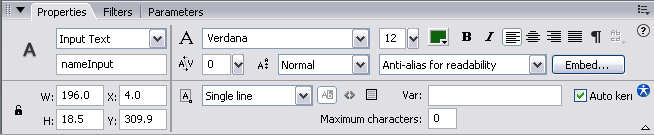
\includegraphics[scale=0.70]{flash-tutorial-images/usage-nameInput-properties.png}
\end{center}


\paragraph{}
Make the second field a Multiline input textfield, with html enabled
and give it the instance name \texttt{commentInput}.


\begin{center}
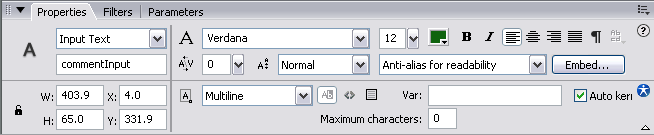
\includegraphics[scale=0.70]{flash-tutorial-images/usage-commentInput-properties.png}
\end{center}



\paragraph{}
Finally, create a button with the label "Submit", and give it the
instance name \texttt{submit}.


\begin{center}
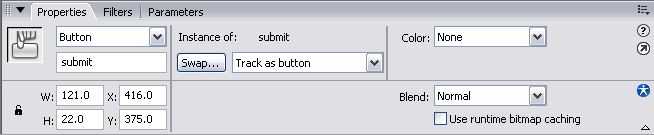
\includegraphics[scale=0.70]{flash-tutorial-images/usage-submit-properties.png}
\end{center}



\paragraph{}
Cozy enough, let's look at what we just did:

\begin{center}
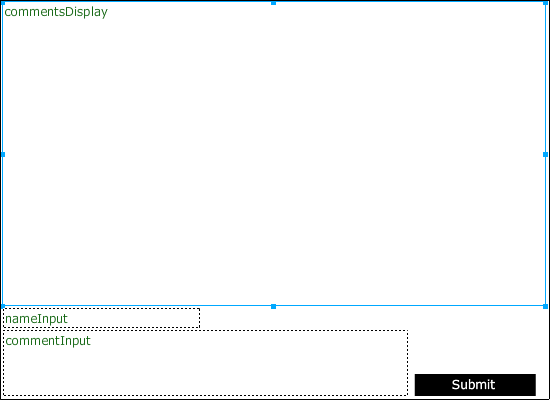
\includegraphics[scale=0.70]{flash-tutorial-images/usage-comments-idle.png}
\end{center}

\section{Setting up a Depot data store}

\paragraph{}
First we have to decide on a prefix for the data store. By convention
we base the directory name on a URL. For this tutorial we'll use
"/com/snepo/examples/flash-comments".


\paragraph{}
On Frame 1 of the main timeline put the following code:

\begin{Verbatim}[frame=single]
import com.snepo.depot.*;

var commentsURL:String = "/com/snepo/examples/flash-comments";
var PO:Depot           = new Depot("localhost", 2323);

function createDirectory(){
   PO.newDirectory ( commentsURL );
   PO.onCreateDirectory = function ( url:String ){
       PO.get ( url );
   }
} 
\end{Verbatim}

\section{The event handlers}

\paragraph{}
Next we need to assign event handlers to a few of Depot's methods to
update, retrieve and display the data from Depot. Add the following
code to the first frame of your movie:

\begin{Verbatim}[frame=single]
PO.onConnect = myOnConnect;
PO.onGet = myOnGet;
PO.onCreate = myOnCreate;
PO.onError  = myOnError;
PO.get(commentsURL);
\end{Verbatim}

\paragraph{}
These event handlers will trigger on certain depot events. The
\texttt{PO.get(commentsURL)} call tells Depot to retrieve all data
from the \texttt{commentsURL} directory.

\paragraph{}
Now remember the first time we try and retrieve data the directory 
may not exist in Depot. The \texttt{myOnError} handler will be called 
if the Depot directory is not found. Add this handler to your code.

\pagebreak

\begin{Verbatim}[frame=single]
function myOnError ( event:String, code:String ){
   if ( code == Errors.NOT_FOUND ){
       createDirectory ();
   }
}
\end{Verbatim}

\paragraph{}
Add the other event handlers underneath the rest of your code. 

\begin{Verbatim}[frame=single]
function myOnConnect(success:Boolean){
     trace("Depot Connect : " +  success);
}
\end{Verbatim}

\paragraph{}
Test your movie and the Output window should show
either "Depot Connect : true" or "Depot Connect : false" depending on
the success of the connection.

\paragraph{}
Add the following code to your movie.

\begin{Verbatim}[frame=single]
function myOnCreate(event:Object){
	trace("Data created");
	PO.get(commentsURL);
}
\end{Verbatim}

This event is invoked whenever a successful
\texttt{DepotInstance.create()} is completed.  Every time you send
data to Depot, it will invoke this handler.

\paragraph{}
In this example, the handler calls \texttt{PO.get(commentsURL);} This
tells depot to retrieve all data from the url commentsURL which we
defined earlier as "/com/snepo/examples/flash-comments". Upon
retrieving that data, Depot will invoke it's \texttt{onGet()} method,
which we defined as \texttt{myOnGet}. Put this code in the
\texttt{myOnGet} function.

\begin{Verbatim}[frame=single]
function myOnGet(results:Array){
	trace(results.length);
}
\end{Verbatim}

\paragraph{}
The \texttt{myOnGet} event handler has an argument called results
which is an array populated by the data retrieved by the last
invocation of \texttt{DepotInstance.get(url)};

\paragraph{}
This handler will trace 0 in flash's Output panel, because we have yet
to store any data in the depot directory.

\paragraph{}
To access the result elements, reference the index in the array that
you want to use. For example, if you wanted the first element
retrieved, the data you need is at \texttt{results[0];} Eg:

\begin{Verbatim}[frame=single]
function myOnGet(results:Array){
	trace("data length : " + results.length);
	trace("first element value : " + results[0]);
}
\end{Verbatim}

\paragraph{}
This will trace undefined because there's no data in the directory.

\section{Storing data}
\paragraph{}
To store a comment, we will need to invoke the \texttt{Depot.create()}
method. This is the method we call to store data. Using the form you
built earlier, we can start storing data by adding the following code
to your flash movie.

\begin{Verbatim}[frame=single]
function store() {
	var body:String = commentInput.text;
	var name:String = "posted by " + nameInput.text;

	var data:Object = {};
	    data.body   = body;
	    data.name   = name;
	
	PO.create(commentsURL, data, "comment");
	
	commentInput.text = "";
	nameInput.text     = "";
}

submit.onPress = store;
\end{Verbatim}

\paragraph{}
This code assigns an \texttt{onPress} handler to your
\texttt{submit} instance that sends the appropriate data to Depot
to be saved.

\paragraph{}
Type "Test Poster" into the \texttt{nameInput} textfield and "Hello,
World" into \texttt{commentInput} and click submit. This will send a
native flash Object with the elements body and name to depot, with the
values of the textfields you typed in.

\paragraph{}
This will then trigger the \texttt{myOnCreate()} function which will
trace "Data Created" in the Output window. As we told
\texttt{myOnCreate()} to call \texttt{myOnGet()}, the following will
appear underneath the last trace message in the output window:

\begin{Verbatim}[frame=single]
data length : 1
first element value : [Object object]
\end{Verbatim}

\paragraph{}
This means that depot has successfully saved your data, and has been
successfully retrieved.  The [Object object] is equal to the data
object we sent to Depot in the \texttt{store()} function, which means
it has 2 fields, one called body, and one called name. Add the
following code to your \texttt{myOnGet()} function and test your
movie.

\begin{Verbatim}[frame=single]
trace("first element name : " + results[0].name);
trace("first element body : " + results[0].body);
\end{Verbatim}

\paragraph{}
You will now see in the Output window:

\begin{Verbatim}[frame=single]
First element name : posted by Test Poster
First element body : Hello, World
\end{Verbatim}


\section{The rest of the code}
\paragraph{}
Now it's time to display the results in the commentsDisplay we  made earlier.

\paragraph{}
Replace your \texttt{myOnGet()} function with the following code: (If
you decided to use a TextArea component from the default flash UI
components, this won't work. You'll need to replace any occurrences of
"htmlText" to "text" in the following block of code)

\begin{Verbatim}[frame=single]
function myOnGet(resultsIn:Array){
   results = resultsIn.reverse(); // show latest comment first
   commentsDisplay.htmlText = "<ul>";
   for(var i:Number = 0; i < results.length; i++){
       var message:String      = results[i].body;
       var name:String         = results[i].name;
       commentsDisplay.htmlText += "<li>" + message + 
                        " <b><i>" + name + 
                        "</i></b></li><br>";
   }
   commentsDisplay.htmlText += "</ul>";
}
\end{Verbatim}

\paragraph{}
This is a standard flash \texttt{for} loop that loops through the
results array and appends the results to a textfield. For readability,
we've made each element in the results array be represented by a list
item.

\paragraph{}
Test your movie and add a few more posts. You should see each new
entry appear at the top of the text field after you submit each
entry. Now go and get some lunch, you deserve it.

\begin{center}
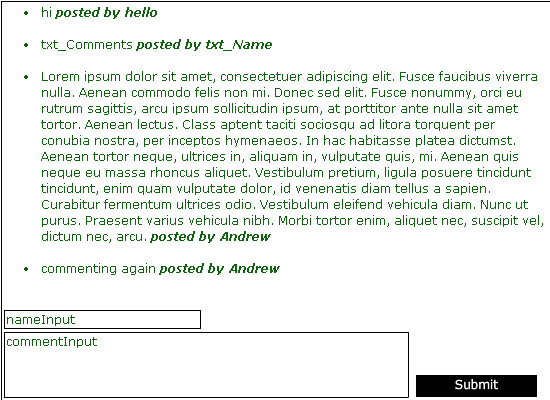
\includegraphics[scale=0.70]{flash-tutorial-images/usage-comments-running.png}
\end{center}



\begin{appendices}


\chapter{Running on the Web}
\label{web.proxy}

\paragraph{}
Flash without a policy file does not allow you to
make HTTP requests to different domains or different ports on the same
domain. Not to worry, like a giant marsupial Depot is lurking just
around the corner with a solution and a furry pouch.
\paragraph{}
The solution is \textbf{proxying}. The web server maps a request to
URL's matching a certain pattern to a different location. The
development server (depot-http) that comes with the Depot install does
this for you. All requests aimed at urls starting with
\texttt{/depot/} are remapped to port 2323.

\begin{Verbatim}[frame=single]
http://localhost:8080/depot/monkey/houseplant
\end{Verbatim}

Becomes 

\begin{Verbatim}[frame=single]
http://localhost:2323/monkey/houseplant
\end{Verbatim}

And nobody is any the wiser. Production web servers like
Apache\footnote{http://apache.org} can be configured to proxy requests
quite easily. Information on setting up Apache to proxy requests to
Depot is included in the Appendices. For development though the
provided depot-http web server should be just fine for all of your
proxying needs.

\paragraph{}
For those of you who would like to deploy to IIS a proxy module is
under development and will be available as soon as possible. 

\paragraph{}
The only code change you need to make to your flash code is included below. 

\begin{Verbatim}[frame=single]
var commentsURL:String;
commentsURL  = "/depot/com/snepo/examples/flash-comments";
var PO:Depot = new Depot("localhost", 8080);
\end{Verbatim}

\paragraph{}
Don't forget to change "localhost" to the production URL when deploying
the SWF to production.


\end{appendices}


\end{document}
